\chapter{Implementierung aufbauend auf bestehenden Technologien, REST API und Continuous Delivery}

\section{Sinatra und PostgreSQL zur Optimiertung des bestehenden Technologiestacks}
Wie bereits in vorangegangenen Kapiteln beschrieben, bieten Microservices die Möglichkeit zum optimierten Einsatz von Technologien. Für die zu entwickelnde Anwendung gab es diverse Optimierungsmöglichkeiten. Die Hauptanwendung ist im Ruby Framework Ruby on Rails\footnote{http://rubyonrails.org} entwickelt worden. Ruby on Rails ist jedoch als Framework zu heavy-weight und mit zu viel Overhead verbunden, als das es sich für einen schnellen, minimalistischen Microservice eignen würde. Ruby on Rails ist an erster Stelle für monolithische Anwendungen entwickelt.~\footcite[][]{rails:doctrine}
Hierbei ist nicht nur die Performance entscheident, sondern auch die Struktur des Codes. Rails als traditionelles Model-View-Controller Framework\footcite[][]{wiki:mvc} eignet sich somit vor Allem auch nicht aufgrund seiner Struktur. Die Rails API Variante\footnote{https://github.com/rails/rails/pull/19832} hingegen hat immer noch zu viel overead für eine optimierte Schnittstelle.

Alternativen bilden sogenannte Microframeworks\footcite[][]{wiki:micro}. Microframeworks zeichnen sich im Gegensatz zu full-stack Frameworks dadurch aus, das viele der Funktionen nicht Teil des mitgelieferten Umfangs sind. In den meisten Sprachen gibt es diverse Microframeworks, wie z.B. Flask\footnote{http://flask.pocoo.org} für Python, Express\footnote{http://expressjs.com} für Node, Sparkjava\footnote{http://sparkjava.com}, oder das Sinatra Framework\footnote{http://www.sinatrarb.com} für Ruby. Die Sprache Go\footnote{https://golang.org} kommt bereits mit gut ausgebauten net/htttp Paketen und umfasst dadurch die meisten üblichen Funktionen schon ohne Framework.

Zwar gibt es Geschwindigkeitsunterschiede in diesen Frameworks\footcite[vgl.][]{frameworks}, im Vergleich zu klassischen full-stack Frameworks sind diese aber unerheblich. Da die Datenbank in der bestehenden Anwendung den größten Flaschenhals bildet (FIX STATS), muss hier nicht zwangsläufig das beste Framework gewählt werden. Stattdessen sollte auf die bestehende Firmenstruktur geachtet werden. Da fast die gesamte Backendtechnologie bisher mit der Programmiersprache Ruby entwickelt ist und es somit keine anderen im Produktionsmodus (FIX IN PRODUCTION) eingesetzt wird, stellt es eine Schwierigkeit dar, eine neue Programmiersprache in die Firma zu integrieren. Vor allem da der neue Microservice auch mit einem komplett eigenen Produktionssetup verbunden ist, stellt eine in der Firma bisher unbekannte Programmiersprache eine ganz eigene Herausforderung dar. Um die Wartbarkeit des Systems hoch zu halten und die Risiken für den Betrieb zu minimieren, entschied ich mich daher auch im neuen Microservice die Programmiersprache Ruby einzusetzen. Da das Framework Ruby on Rails überproprtioniert ist und nicht den Anforderungen entspricht, entschied ich mich für den Einsatz des Ruby Frameworks Sinatra. 
Sinatra ist nach Ruby on Rails das mit Abstand beliebteste Ruby Framework\footcite[vgl.][]{ruby2015} und wird daher von den meisten Ruby Web Tools unterstützt.

Wie bereits erwähnt, ist Sinatra ein sogenanntes Microframework. Sinatra selbst bringt also nicht viel Logik, die die Entwicklung beeinflusst. Einige Dinge die Sintra erleichtert, sind vor Allem das Routing. Hier kann schnell eine Routing Struktur erschaffen werden, die Definition von Routen und deren Antworten ist sehr komfortabel und schnell eingerichtet. Sinatra ist vor Allem auch nicht darauf ausgelegt in Antworten HTML zu rendern, so kann leicht eine JSON Response definiert werden.
Eine Route zum Anlegen von Resourcen kann demnach so definiert werden:
\begin{lstlisting}[language=Ruby]
class SomeController < Sinatra::Base
  post '/resources' do
    data = JSON.load(request.body.read)
    [...] # some actions to save the resource
    # return appropriate 201 code and json with access key
    [201, { data: { key: some_key  } }.to_json }]
  end
end
\end{lstlisting}

Weiterhin erleichtert Sinatra das Betreiben eines Webservers und bietet eine Schnittstelle zum Ruby Standard Webserver Interface Rack\footnote{http://rack.github.io}. Hier wird dem Entwickler viel Arbeit abgenommen. Viele Tools zum Betreiben von Webservices, z.B. im Bereich des Monitorings oder des Loggings unterstützen ebenfalls das Sinatra Framework. So bringt Sinatra also nicht viel overhead out of the box, bringt aber die Möglichkeit zur Nutzung vieler praktischer Erweiterungen.

Da die Datenbank das scheinbar größte Problem der Performance in der bestehenden Anwendung bildet, ist es hier dringend notwendig die eingesetzte Technologie zu überdenken. Zwar ist MongoDB von der Idee her keine schlechte Wahl für die Userprofile, die Art wie Profildaten abgefragt werden, passt aber nicht gut zum dokumentorientierten Ansatz von MongoDB.
Die Schemalosigkeit von MongoDB in Zusammenarbeit mit den recht variablen Profilen war ursprünglich der Hauptgrund diese Technologie einzusetzen. Userprofile sind startk unterschiedlich, viele mit ja beantworteten Fragen führen zu weiteren Fragen (z.B. ``Haben Sie Kinder?'', ``Wie viele Kinder haben Sie?'', ``Wie alt ist Kind x?''). Hierbei bietet es sich durchaus an MongoDB mit seiner Embedded Document Struktur zu benutzten, statt unzählige 1 zu n Beziehungen zu verwalten. Die Art der Abfrage ist aber für die Geschwindigkeit unterscheident. Hier verspricht die Struktur von MongoDB Geschwindigkeitsvorteile, wenn man einzelne Dokumente aus der Datenbank erhalten möchte. So kann zum Beispiel die Struktur einer Powerpoint Struktur wie folgt abgebildet werden.
\begin{lstlisting}[language=Ruby]
{
    presentationId: 1,
    title: "A Presentation",
    author: "me",
    slides: [
        {
            slideId: 1,
            slideOrder: 1,
            elements: [
                {
                    elementId: 1,
                    elementXPos: 100,
                    ...
                },
                ...
                }
            ]
        },
        ...
    ]
}
\end{lstlisting}
Eine Präsentation kann nun mit nur einer Abfrage, ohne jegliche Joins aus der Datenbank geladen werden. Die ganze Präsentation kann vorgerendered werden und die Anwendung zur Erstellung oder Präsentation von Präsentationen ohne weiteres Nachladen genutzt werden. Hier liegt MongoDB's Stärke: Strukturen können in ihrer natürlichen Form abgebildet werden und dokumentorientiert schnell aus der Datenbank geladen werden.
So ist auch der Aufbau der Profile konzipiert worden. Nun kommt es aber verhältnismäßig selten vor, dass ein gesamtes Userprofil geladen werden muss. Dies ist nur der Fall, wenn User ihr Profil anpassen wollen.
Wesentlich öfter hingegen werden Userprofile abgefragt um User zu Umfragen einzludaen. Hier interessiert aber nie ein ganzer Nutzer, sondern lediglich ein Querschnitt über alle Nutzer. Queries sehen in der Regel wie folgt aus:
\begin{lstlisting}[language=Ruby]
{
    "profile.participations.response_rate.value": {
        "$lt": 0.3
    },
    "profile.basic.locale.value": {
        "$in": ["de", "de-AT"]
    },
    "profile.basic.age.value": {
        "$gt": 21,
        "$lte": 100
    }
}
\end{lstlisting}

Hier wird auf eine verhältnismäßig geringe Zahl von Profilfelder, meist weniger als 10, über die gesamte Population gequeried. Weiterhin werden dann nicht gesamte Nutzerobjekte zurückgegeben, sondern lediglich die Anzahl der passenden Nutzer, deren Ids oder Antwortraten. Die MongoDB query Struktur ist dafür einfach nicht optimiert. Hinzu kommt die extreme Verschachtelung der Datenstruktur. So werden nicht nur Profildaten wie Kinder in ein Subdokument gruppiert, es gibt auch noch thematische Unterteilungen der Profildaten, ``basic'' für die allgemeinen personenbezogenen Daten, ``basic.education'' für Daten über den Bildungsgrad.
Hinzu kommt die relative Größe der Datenbank. Knapp 400.000 Userdaten mit bis zu 176 ausgefüllten Prodfilfeldern passen aktuell nicht einmal mehr in den Arbeitsspeicher der Server. Nicht alle Felder können logischerweise mit Indexen abgedeckt werden, die relative Verteilung der Queries umfasst aber alle Felder. Zwar gibt es besondere Häufungen der Queries bei bestimmten Feldern und diese sind auch durch Indexes abgedeckt, vor Allem aber die Queries auf die anderen Felder verlangsamen die Anwendung nicht unerheblich.
Aufgrund der offensichtlichen Mängel bot es sich an, die Datenbanktechnologie zu wechseln und stattdessen eine SQL Datenbank zu verwenden. Im Gegensatz zum Wechsel der Programmiersprache, stellt der Einsatz einer anderen Datenbanktechnologie im konkreten Fall keine große Hürde dar. Im Betrieb besteht bereits eine MySQL\footnote{http://www.mysql.com} Datenbank als Data Warehouse und eine PostgreSQL\footnote{http://www.postgresql.org} Datenbank für eine für einen Kunden betriebene Anwendung. Daher besteht Erfahrung sowohl in der Entwicklung mit, als auch dem Betrieb von SQL Datenbanken.

Testing, Git, CI, Deployment!?

\section{Schaffung einer standardisierten REST Schnittstelle}
Einen entscheidenen Unterschied zwischen Microservice Architektur und monolithischer Entwicklung, bildet die Schnittstelle zwischen den Anwendungsteilen. Während im Monolithen simple code calls stattfinden, muss für die Kommunikation zwischen verschiedenen Servies zunächst ein geeignetes Protokoll zum Austausch gefunden werden.

\section{Integration des Microservices in den Monolithen}
Wie bereits im vorangegangenen Kapitel beschrieben, beschloss ich mich die neue Microservice Anwendung mit Hilfe des Flipper Gems parallel zu betreiben. Anhand der abstrahierten Schnittstelle des QueryExecuters, wird entschieden ob ein Query auf der alten Datenbank oder dem neuen Service stattfindet.
\begin{figure}[h]
    \centering
    \caption{Klassendiagramm zur Verteilung zwischen bestehendem und neu geschaffenem Code}
    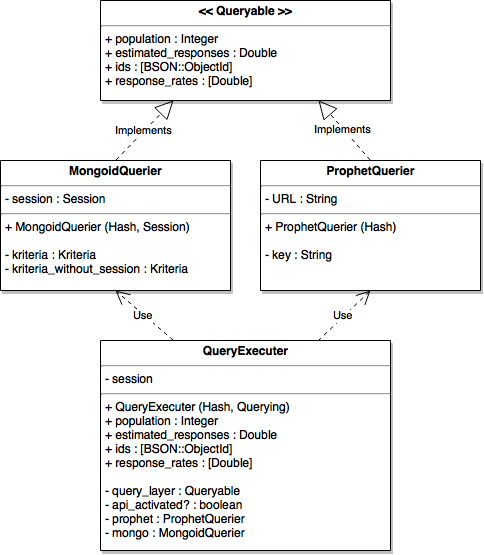
\includegraphics[scale=0.6]{klassendiagramm}
\end{figure}

Ist der Flipper aktiviert, wird zunächst ein per POST ein Query an den Service übertragen. Im Hintergrund initiiert der Service dann ein parsen, übersetzen und abarbeiten der Query, dies geschieht asynchron. Zunächst wird die Query in Redis gespeichert und der generierte Zugriffsschlüssel zurückgegeben.
Anhand dieses Schlüssels kann die Hauptanwendung dann die freigegebenen Ergebnisse des Querys, wie die Ids der zutreffenden User, abfragen. Der Ablauf kann wie folgt visualisiert werden:

\begin{figure}[h]
    \centering
    \caption{Sequenzdiagramm zum Profilqueryen bei aktiviertem Flipper}
    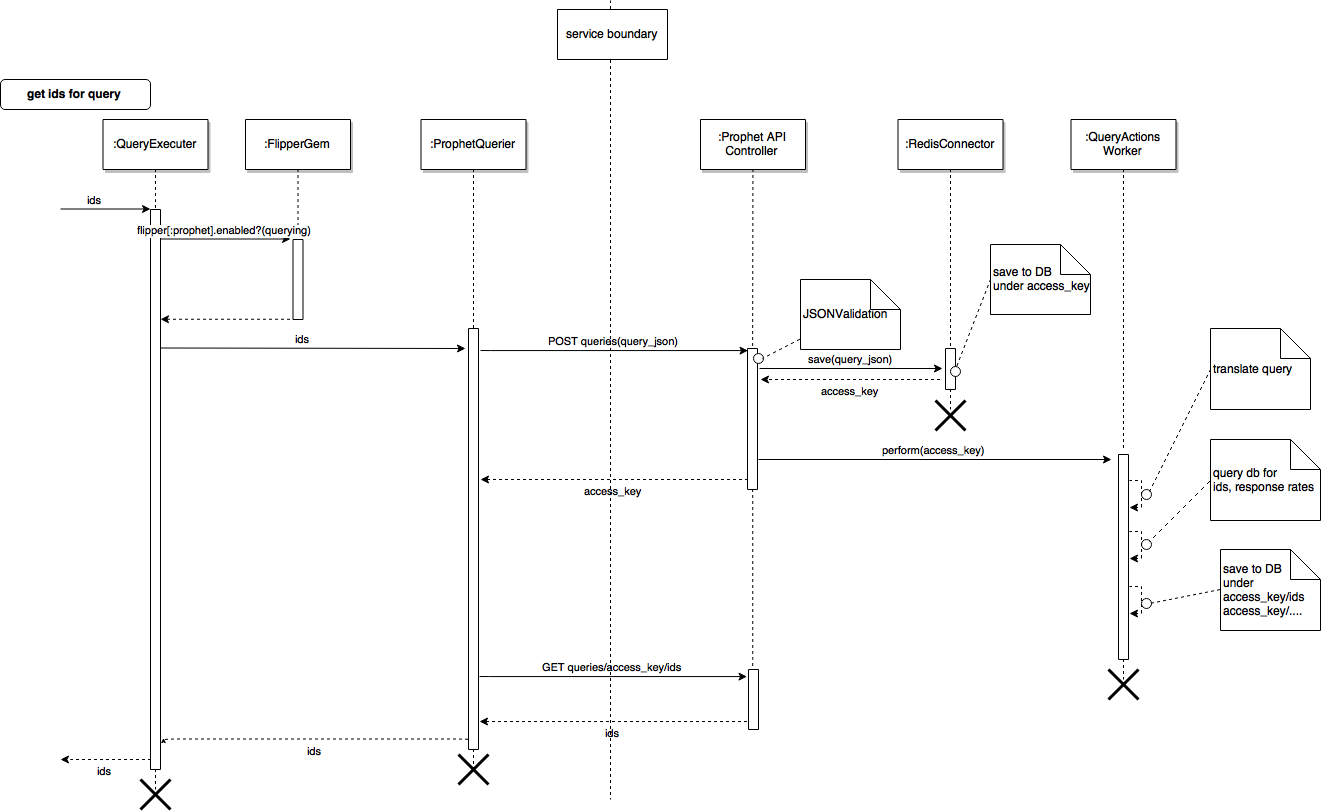
\includegraphics[width=\textwidth]{prophet_sequenz}
\end{figure}

\section{Betrieb der Anwendung auf AWS - Betreuung, Monitoring und Scaling}
Wie bereits beschrieben, bilden die Skalierungsmöglichkeiten von Microservices einen großen Vorteil des Architekturstils. Um diesen optimal ausnutzen zu können, bietet es sich an ein dynamisches Hosting einzurichten. Hier gibt diverse Lösungen, die alle einen ähnlichen Funktionsumfang bieten. Zu nennen sind hier insbesondere Amazon Web Services (AWS), Google App Engine und Heroku. Da die AWS eine der reifesten Platformen ist, beschloss ich für den Microservice AWS als Hoster zu wählen.
Auf AWS nutze ich Amazon Beanstalk zum Betreiben der Anwendung. Beanstalk nutzt intern EC2 Instanzen, baut aber eine eigene Konfigurationsschicht darauf auf. Daher muss keine gesamte virtuelle Maschine betrieben werden, sondern die Anwendung kann leicht über ein Konfigurationsinterface gesteuert werden. (FIX BILD??)
AWS Beanstalk ist selbst mit keinen Kosten verbunden, man bezahlt nur für die von Beanstalk genutzten Resourcen, also die genutzten EC2 Instanzen und der reine Speicherverbrauch der Anwendung auf AWS S3. Die weiteren von der Anwendung benötigten Resourcen sind zum Einen eine PostgreSQL Datenbank und der Key-Value Store Redis. Hierfür bietet Amazon jeweils gesonderte Service zum Betrieb. Relationale Datenbanken können über den Amazon Relational Database Service (RDS) genutzt werden, Redis wird über Amazon ElastiCache angeboten. Beide Services bieten ebenso wie Beanstalk gute Skalierungsmöglichkeiten.
Entscheidend ist ebenfalls das Monitoring. Skylight und Bugsnag als Integration in bestehende Firmenteile.